\begin{framed}

Objetivos:
\begin{itemize}
    \item Repasar la descripción de fluidos mediante ecuaciones diferenciales.
    \item Repasar las leyes de conservación.
\end{itemize}

Contenidos:
\begin{itemize}
    \item Introducción y generalidades.
    \item Repaso: cinemática de una partícula de fluido.
    \item Repaso: Ecuaciones diferenciales de conservación. 
    \begin{itemize}
        \item Masa: Continuidad.
        \item Momentum: Navier-Stokes.
        \item Condiciones de contorno.
    \end{itemize}
\end{itemize}

Bibliografía:
\begin{itemize}
    \item White, F. M. (2008) Mecánica de Fluidos. McGraw-Hill. Sexta edición. Secciones 4.1-4.4
    \item Fox, R. W., Pritchard, P. J. y McDonald, A. T. (2009) Introduction to Fluid Mechanics. John Wiley \& Sons. Secciones 5.1-5.4
\end{itemize}
\end{framed}

En esta primera clase estudiaremos el análisis diferencial del movimiento de un fluido. 
Para esto, iniciaremos viendo como se describe el movimiento de un elemento diferencial de fluido, para luego aplicar las leyes de conservación de masa, cantidad de movimiento, y energía sobre el elemento diferencial.
 Este material fue visto en el curso Mecánica de Fluidos General, sin embargo, lo repasamos para estar en la misma página con respecto a lo que viene hacia adelante.

\section*{Elemento diferencial en movimiento}
Digamos que tenemos un flujo y que somos capaces de hacer un pequeño cuadrado con tinta al tiempo $t=0$.
Este pequeño cuadrado servirá como nuestro elemento diferencial a analizar.
Digamos que esperamos una pequeña cantidad de tiempo $\delta t$ y le sacamos una foto \mbox{?`}Qué ocurrió con el cuadrado que dibujamos? Algo como lo que muestra la Figura \ref{fig:elemento_diferencial}
%
\begin{figure}[h!]
\centering
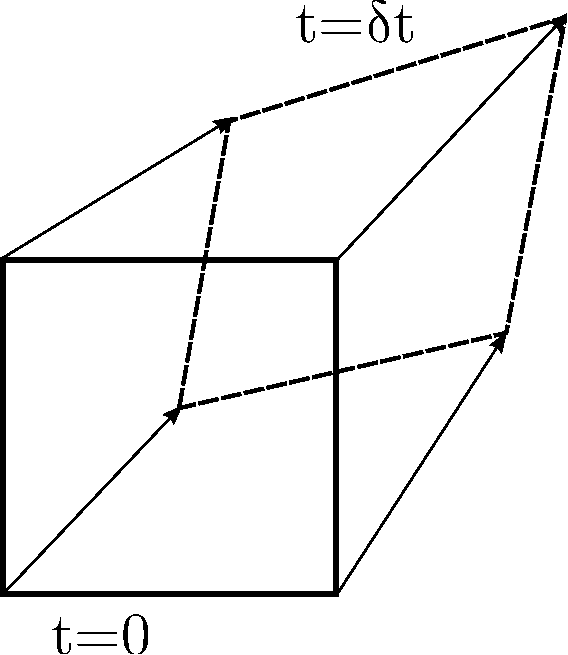
\includegraphics[width=0.4\textwidth]{clase01/elemento_diferencial.pdf}
\caption{Deformación y traslación de un elemento diferencial tras un tiempo $\delta t$}
\label{fig:elemento_diferencial}
\end{figure}

La razón por la que el elemento de fluido de la Figura \ref{fig:elemento_diferencial} se deformó es que la velocidad no es constante dentro del mismo. 
En la figura, las flechas representan el cambio de posición de las esquinas en el tiempo $\delta t$. 
Al ser la misma cantidad de tiempo $\delta t$ en los cuatro casos, las flechas nos entregan una idea de la velocidad en esos puntos, la cual es distinta en cada caso.
De hecho, si $\delta t=1$s, las flechas serían exactamente la velocidad. 

De esta forma, podemos concluir que existe un campo de velocidad $\mathbf{V}(\mathbf{x},t) = (u(\mathbf{x},t),v(\mathbf{x},t),w(\mathbf{x},t))$, donde $\mathbf{x}=(x,y,z)$, que puede ir variando en el espacio y tiempo.

\subsubsection*{Campo de velocidades}
Nuestro modelo se basa en considerar el fluido como un continuo. 
Por lo tanto, en vez de tener velocidades discretas de cada molécula de agua, analizamos el comportamiento promedio, y podemos representar la velocidad como una función continua:
%
\begin{equation}
\mathbf{V}(\mathbf{x},t) = u(\mathbf{x},t)\ihat+v(\mathbf{x},t)\jhat+w(\mathbf{x},t)\khat,
\end{equation}
%
donde, como antes, $\mathbf{x} = (x,y,z)$. 

Se habrán dado cuenta que la partícula de fluido se mueve con el fluido, por lo tanto, $\mathbf{x}=\mathbf{x}(t)$. 
Estudiemos la aceleración de la partícula.
Si el elemento de fluido estuviese detenido, simplemente $\mathbf{a}=\frac{\partial \mathbf{V}}{\partial t}$ nos entregaría la aceleración, sin embargo, al estar moviéndose con el fluido, utilizaremos la notación $\frac{D}{Dt}$, que se conoce como derivada material o total:
%
\begin{equation}\label{eq:acel}
\mathbf{a} = \frac{D\mathbf{V}}{Dt} = \frac{Du}{Dt}\ihat+\frac{Dv}{Dt}\jhat+\frac{Dw}{Dt}\khat.
\end{equation}
%
Veamos lo que ocurre en el eje $x$. 
Por regla de la cadena, queda:
%
\begin{equation}
\frac{Du}{Dt} = \frac{\partial u}{\partial x}\frac{Dx}{Dt} +\frac{\partial u}{\partial y}\frac{Dy}{Dt} +\frac{\partial u}{\partial z}\frac{Dz}{Dt}+ \frac{\partial u}{\partial t}\frac{Dt}{Dt}
\end{equation}
%
pero,
\begin{align}
\frac{Dx}{Dt} &= u \nonumber\\
\frac{Dy}{Dt} &= v \nonumber\\
\frac{Dz}{Dt} &= w 
\end{align}
%
y llegamos a
%
\begin{equation}
\frac{Du}{Dt} = u\frac{\partial u}{\partial x} + v\frac{\partial u}{\partial y} + w\frac{\partial u}{\partial z} + \frac{\partial u}{\partial t}
\end{equation}
%
En 3 dimensiones, esto es
%
\begin{equation}\label{eq:der_mat}
\mathbf{a} = \frac{D\mathbf{V}}{Dt} = \frac{\partial \mathbf{V}}{\partial t} + u\frac{\partial \mathbf{V}}{\partial x} + v\frac{\partial \mathbf{V}}{\partial y} + w\frac{\partial \mathbf{V}}{\partial z} = \underbrace{\frac{\partial \mathbf{V}}{\partial t}}_\text{local} + \underbrace{(\mathbf{V}\cdot\nabla)\mathbf{V}}_\text{convectiva},
\end{equation}
%
donde el primer término se conoce como aceleración local, y el segundo como aceleración convectiva.
Noten que un elemento de fluido se puede estar acelerando incluso en una situación estacionaria (donde $\partial \mathbf{V}/\partial t=0$).

\subsubsection*{Movimiento de un elemento diferencial}
La Figura \ref{fig:elemento_diferencial} muestra como un elemento de fluido cuadrado se mueve y deforma. 
Uno puede imaginar que mientras más complicado el campo de velocidad, se hace más difícil de entender la deformación.
Para facilitar el análisis, la Figura \ref{fig:deformacion} describe el movimiento y deformación en cuatro partes: traslación, deformación lineal, rotación y deformación angular.
%
\begin{figure}[h!]
\centering
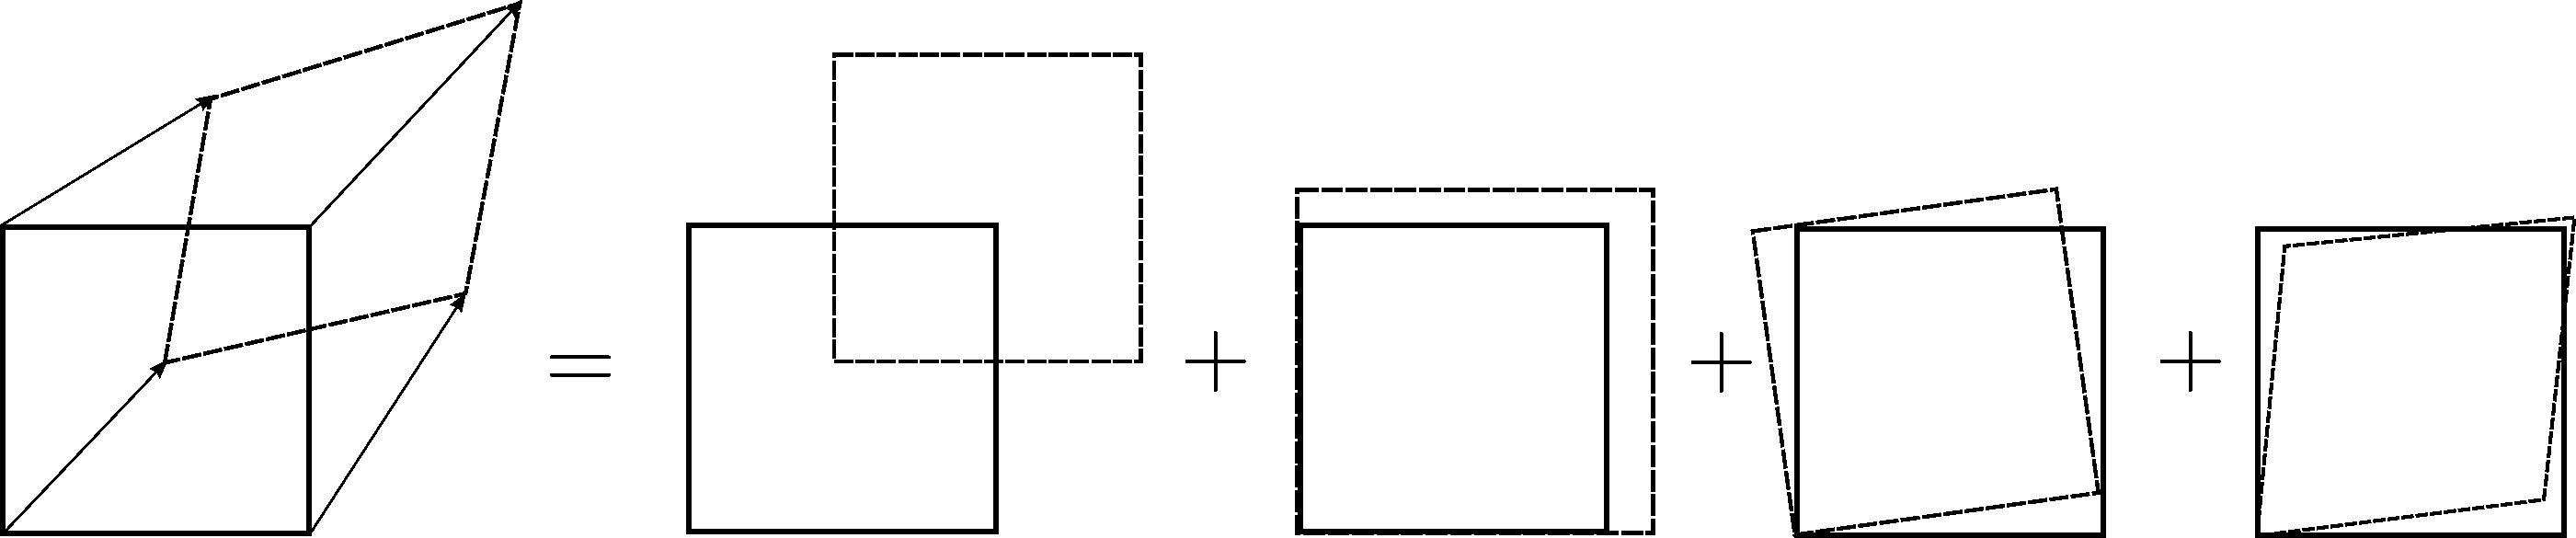
\includegraphics[width=\textwidth]{clase01/deformacion.pdf}
\caption{Traslación, deformación lineal, rotación y deformación angular de un elemento de fluido}
\label{fig:deformacion}
\end{figure}
%
Analicemos cada una de estas.

\paragraph{Traslación y deformación lineal.}
La traslación como aparece en el primer término de la Figura \ref{fig:deformacion} ocurre cuando la velocidad del fluido es constante dentro del volúmen.
Ese es un caso muy simple y poco interesante 
\mbox{?`}Qué ocurre cuando no es así? 
Probemos con el caso unidimensional de la Figura \ref{fig:deformacion_lineal}:
%
\begin{figure}[h!]
\centering
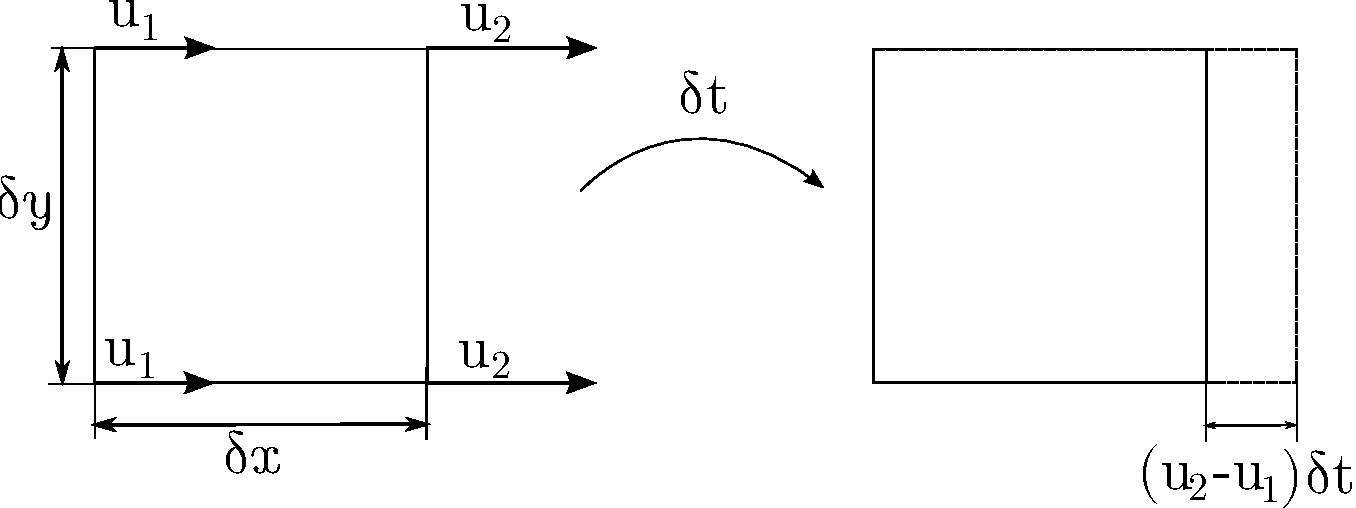
\includegraphics[width=0.7\textwidth]{clase01/deformacion_lineal.pdf}
\caption{Deformación lineal en el eje x.}
\label{fig:deformacion_lineal}
\end{figure}

El cuadrado en la Figura \ref{fig:deformacion_lineal} es un elemento diferencial, por lo tanto, $\delta x$ es pequeño, y las esquinas están muy cerca entre si.
Por esto, una expansión de Taylor centrada en la locación de $\mathbf{u}_1$ nos entregará una buena aproximación de la velocidad $\mathbf{u}_2$:
%
\begin{equation}
\mathbf{u}_2 = \mathbf{u}_1 + \frac{\partial \mathbf{u}}{\partial x}\delta x + \frac{1}{2}\frac{\partial^2 \mathbf{u}}{\partial x^2}\delta x^2 + \frac{1}{6}\frac{\partial^3 \mathbf{u}}{\partial x^3}\delta x^3 + \dots
\end{equation}
%
Pero ya dijimos que $\delta x$ es pequeño, lo que implica que $\delta x^2$ es aún más pequeño, y así todos los términos de orden superior.
Si despreciamos todos esos términos, podemos decir que
%
\begin{equation}\label{eq:u_lineal}
\mathbf{u}_2 \approx \mathbf{u}_1 + \frac{\partial \mathbf{u}}{\partial x}\delta x,
\end{equation}
%
es una buena aproximación.
Manipulando la Ec. \eqref{eq:u_lineal} podemos llegar a
%
\begin{equation}
(\mathbf{u}_2-\mathbf{u}_1)\delta t=\frac{\partial \mathbf{u}}{\partial x}\delta x\delta t,
\end{equation}
%
lo que coincide con el estiramiento del elemento diferencial en la Figura \ref{fig:deformacion_lineal}.
Podemos obtener el cambio en volumen ($\delta \vol$) al multiplicar $(\mathbf{u}_2-\mathbf{u}_1)\delta t$ por la sección transversal ($\delta y\cdot \delta z$), por lo tanto,
%
\begin{align}
\delta \vol &= \frac{\partial \mathbf{u}}{\partial x} \delta x\delta y\delta z\delta t, \text{ y} \nonumber \\
\frac{\delta \vol}{\delta t} &= \frac{\partial \mathbf{u}}{\partial x} \vol,
\end{align}
%
donde $\vol = \delta x\delta y\delta z$ es el volumen original del elemento de fluido.
Así, llegamos a que el cambio de volumen por unidad de volumen es
%
\begin{equation}
\frac{1}{\vol}\frac{\delta \vol}{\delta t} = \frac{\partial \mathbf{u}}{\partial x},
\end{equation}
%
En tres dimensiones, la derivación equivalente nos deja:
%
\begin{equation}\label{eq:dil_vol} 
\frac{1}{\vol}\frac{\delta \vol}{\delta t} = \frac{\partial u}{\partial x} +\frac{\partial v}{\partial y} +\frac{\partial w}{\partial z}  = \nabla \cdot \mathbf{V}.
\end{equation}

El término al lado izquierdo de la Ec. \eqref{eq:dil_vol} se conoce como dilatación volumétrica.
La Ec. \eqref{eq:dil_vol} nos muestra que la divergencia del campo de velocidad nos entrega información muy valiosa, ya que está relacionado con el cambio volumétrico en el tiempo:
%
\begin{itemize}
\item[$\nabla \cdot \mathbf{V} > 0$:] el fluido se está dilatando. 
\item[$\nabla \cdot \mathbf{V} < 0$:] el fluido se está comprimiendo. 
\item[$\nabla \cdot \mathbf{V} = 0$:] no hay cambio en volumen. Ejemplo: flujo incompresible. 
\end{itemize}

\paragraph{Rotación y deformación angular.}
La rotación y deformación angular ocurre por la diferencia de velocidad normal a la línea que une las esquinas del elemento diferencial, como lo muestra la Figura \ref{fig:deformacion_angular}.

\begin{figure}[h!]
\centering
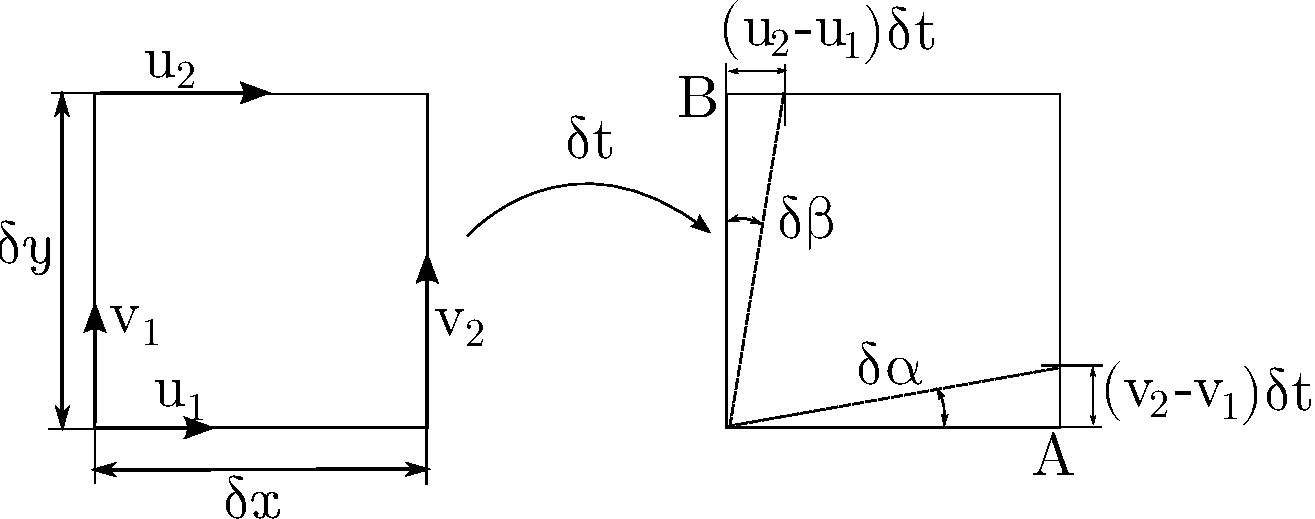
\includegraphics[width=0.7\textwidth]{clase01/deformacion_angular.pdf}
\caption{Deformación angular en el eje z.}
\label{fig:deformacion_angular}
\end{figure}

De la misma manera que para la deformación lineal, al ser $\delta x$ y $\delta y$ pequeños, la serie de Taylor truncada en el término de primer orden nos entrega una buena aproxiamción y llegamos a que
%
\begin{align}
(u_2-u_1)\delta t &\approx \frac{\partial u}{\partial y} \delta y\delta t \nonumber \\
(v_2-v_1)\delta t &\approx \frac{\partial v}{\partial x} \delta x\delta t.
\end{align}
%
Por otra parte, al ser $\delta t$ pequeño, se forman dos triángulos rectángulos, donde, por simple trigonometría:
%
\begin{align}
\tan (\delta \alpha) &= \frac{\partial v}{\partial x} \delta x\delta t\frac{1}{\delta x}\nonumber \\
\tan (\delta \beta) &= \frac{\partial u}{\partial y} \delta y\delta t\frac{1}{\delta y}.
\end{align}
%
Los ángulos $\delta \alpha$ y $\delta \beta$ son muy pequeños, por lo tanto es válida la aproximación de ángulo pequeño ($\tan (\delta \alpha)\approx\delta\alpha$,$\tan (\delta \beta)\approx\delta\beta$), lo que nos entrega:
%
\begin{align}\label{eq:triangulo}
\delta \alpha &= \frac{\partial v}{\partial x} \delta x\delta t\frac{1}{\delta x}\nonumber \\
\delta\beta &= \frac{\partial u}{\partial y} \delta y\delta t\frac{1}{\delta y}.
\end{align}

La velocidad angular de los puntos $A$ y $B$ están dados por 
%
\begin{align}\label{eq:omega}
\Omega_A &= \lim_{\delta t\to 0}\frac{\delta \alpha}{\delta t} \nonumber \\
\Omega_B &= \lim_{\delta t\to 0}\frac{\delta \beta}{\delta t},
\end{align}
%
donde, según la Figura \ref{fig:deformacion_angular}, $\Omega_A$ gira en dirección $\khat$ y $\Omega_B$ en dirección $-\khat$.
Reemplazando la Ec. \eqref{eq:triangulo} en la Ec. \eqref{eq:omega}, se cancela el término $\delta t$ y obtenemos
%
\begin{align}
\Omega_A &= \frac{\partial v}{\partial x}\nonumber \\
\Omega_B &= -\frac{\partial u}{\partial y}.
\end{align}

El punto más representativo del elemento de fluido es su centro geométrico, el cual gira con una velocidad angular igual al promedio entre $\Omega_A$ y $\Omega_B$. 
De esta forma, podemos decir que el elemento de fluido esta rotando con velocidad 
%
\begin{equation}\label{eq:omega_z}
\Omega_z = \frac{\Omega_A+\Omega_B}{2} = \frac{1}{2}\left(\frac{\partial v}{\partial x}-\frac{\partial u}{\partial y}\right).
\end{equation}

Haciendo el análisis equivalente en las otras dos dimensiones llegamos a
%
\begin{align}
\Omega_x &= \frac{1}{2}\left(\frac{\partial w}{\partial y} -\frac{\partial v}{\partial z}\right) \nonumber \\
\Omega_y &= \frac{1}{2}\left(\frac{\partial u}{\partial z} -\frac{\partial w}{\partial x}\right).
\end{align}
%
Nos conviene definir un vector rotación $\boldsymbol{\Omega}$, tal que
%
\begin{equation}
\boldsymbol{\Omega} = \Omega_x \ihat + \Omega_y \jhat + \Omega_z \khat = \frac{1}{2}\left(\nabla\times\mathbf{V}\right),
\end{equation}
%
y por comodidad, hablaremos de la vorticidad $\boldsymbol{\omega}$
%
\begin{equation}\label{eq:vorticidad}
\boldsymbol{\omega} = 2\boldsymbol{\Omega} = \nabla\times\mathbf{V}.
\end{equation}

En la segunda parte del curso revisaremos el concepto de vorticidad más en profundidad.
Es importante no confundir la rotación de un elemento de fluido con un flujo que rota: es perfectamente posible que un elemento de fluido tenga una trayectoria curva sin rotar o deformarse angularmente (un ejemplo de esto de el punto vórtice, que conocerán pronto).

\section*{Leyes de conservación}

Las ecuaciones diferenciales que comúnmente utilizamos en mecánica de fluidos no son más que la aplicación de las leyes de conservación en el elemento diferencial de fluido de la Figura \ref{fig:elemento_diferencial}.
Estas leyes de conservación son tres: masa, cantidad de movimiento y energía.
En esta clase revisaremos las dos primeras, que son con las que trabajaremos en este curso. 
No iremos al detalle de la derivación, pues ya fue hecho en el curso anterior, sin embargo revisaremos los principales resultados.

\subsection*{Conservación de masa}

Esta es la más intuitiva de las leyes de conservación. 
Imaginemos que pintamos la región dentro del elemento de fluido, y esperamos un tiempo $\delta t$: la cantidad de moléculas pintadas sigue siendo la misma.
En otras palabras, la cantidad de masa dentro del elemento de fluido no puede cambiar: $Dm/Dt=0$.
Tenemos todos los elementos para hacer una rápida derivación de la ecuación de continuidad, la cual aparece en el libro \emph{Hydrodynamics} de Horace Lamb (un clásico, para quien esté interesado):
%
\begin{align}
\frac{Dm}{Dt} &= \frac{D(\rho\vol)}{Dt} = \rho\frac{D\vol}{Dt} + \vol\frac{D\rho}{Dt} = 0 \left/\cdot\frac{1}{\vol}\right. \nonumber \\
\Rightarrow & \rho \underbrace{\frac{1}{\vol}\frac{D\vol}{Dt}}_\text{$=\nabla\cdot\mathbf{V}$} + \frac{D\rho}{Dt} = 0,
\end{align}
%
donde $\rho$ es la densidad, y usamos la Ec. \eqref{eq:dil_vol} sabiendo que $D\vol/Dt=D\delta\vol/Dt$. 
Si expandemos la divergencia y la derivada material (usando la Ec. \eqref{eq:der_mat}), llegamos a:
%
\begin{equation}
\rho\left(\frac{\partial u}{\partial x} + \frac{\partial v}{\partial y} + \frac{\partial w}{\partial z}\right) + \frac{\partial \rho}{\partial t} + u\frac{\partial \rho}{\partial x} + v\frac{\partial \rho}{\partial y} +w\frac{\partial \rho}{\partial z} = 0,
\end{equation}
%
y recombinando los términos obtenemos la forma final de la ecuación de continuidad:
%
\begin{equation}\label{eq:continuidad}
\frac{\partial \rho}{\partial t} + \frac{\partial (\rho u)}{\partial x} + \frac{\partial (\rho v)}{\partial y} + \frac{\partial (\rho w)}{\partial z} = \frac{\partial \rho}{\partial t} + \nabla\cdot(\rho\mathbf{V})= 0
\end{equation}

Un caso interesante que nos entrega la Ec. \eqref{eq:continuidad} es el flujo incompresible, donde la densidad es constante en el tiempo y espacio. 
Por lo tanto, la derivada temporal es cero, y $\rho$ puede salir de la derivada espacial, quedando $\nabla\cdot\mathbf{V}=0$.
Este resultado coincide con el análisis que hicimos de la dilatación volumétrica en la Ec. \eqref{eq:dil_vol}.

\subsection*{Conservación de cantidad de movimiento}

La ley de conservación de la cantidad de movimiento no es más que la segunda ley de Newton: si hay cambios en la cantidad de movimiento, es porque una fuerza resultante total no nula actuando sobre el elemento de fluido.
Matemáticamente, esto es:
%
\begin{equation}\label{eq:cant_mov}
\frac{D\mathbf{p}}{Dt} = \sum\mathbf{F}.
\end{equation}

\begin{figure}[h!]
\centering
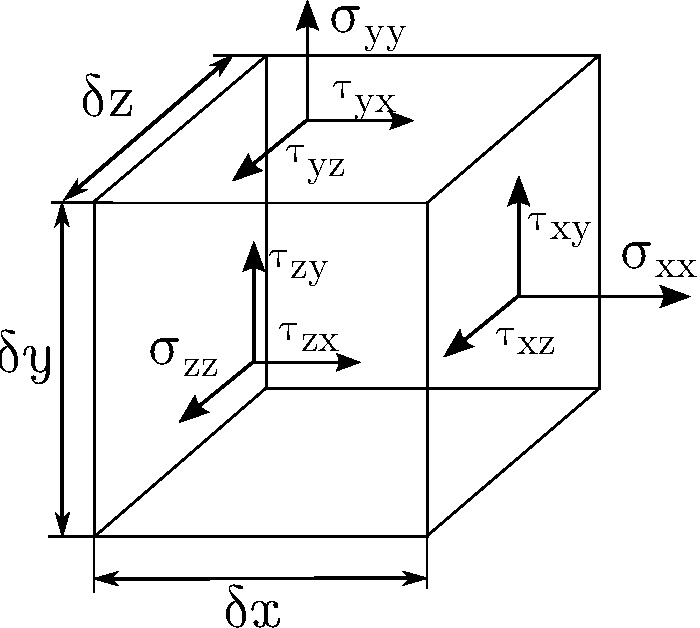
\includegraphics[width=0.4\textwidth]{clase01/cant_mov.pdf}
\caption{Fuerzas sobre un elemento de fluido.}
\label{fig:cant_mov}
\end{figure}

La derivación en este caso es larga, y no iremos en tanto detalle, pero presentaremos los principales pasos a continuación.
En el caso del elemento de fluido de la Figura \ref{fig:cant_mov}, éste está sujeto a los esfuerzos normales $\sigma_{ij}$ y cortantes $\tau_{ij}$ en la superficie.
Para mayor claridad en la Figura \ref{fig:cant_mov}, no dibujamos los esfuerzos en las caras posteriores, pero según la convención de signo, los esfuerzos apuntan en la dirección contraria.
Esto implica que la suma vectorial resulta en la diferencia entre cada uno de los esfuerzos $\tau_{ij}$ y $\sigma_{ij}$, evaluados en la cara frontal y posterior.

Considerando que $\delta x$, $\delta y$, y $\delta z$ son pequeños, podemos usar una expansión de Taylor truncada al término de primer orden para encontrar el cambio de los esfuerzos a través del elemento de fluido.
Por ejemplo, el caso de la cara normal al eje $x$:
%
\begin{align}
\sigma_{xx}(x+\delta x)-\sigma_{xx}(x) &\approx \frac{\partial \sigma_{xx}}{\partial x}\delta x \nonumber \\
\tau_{xy}(x+\delta x)-\tau_{xy}(x) &\approx \frac{\partial \tau_{xy}}{\partial x}\delta x \nonumber \\
\tau_{xz}(x+\delta x)-\tau_{xz}(x) &\approx \frac{\partial \tau_{xz}}{\partial x}\delta x,
\end{align}
%
lo que es fácilmente extendible a las caras normales a $y$ y $z$. 
Multiplicando los esfuerzos por las áreas correspondientes para convertirlos en fuerzas, y considerando la componente gravitacional ($m\mathbf{g}=\rho\vol\mathbf{g}$), obtenemos la siguiente expresión para la suma de fuerzas:
%
\begin{equation}\label{eq:suma_F}
\sum F_x = \frac{\partial \sigma_{xx}}{\partial x}\delta x\delta y \delta z + \frac{\partial \tau_{yx}}{\partial y} \delta x \delta y \delta z + \frac{\partial \tau_{zx}}{\partial z} \delta x \delta y \delta z + \rho \vol g_x,
\end{equation}
%
donde $\delta x \delta y \delta z=\vol$.

Por otra parte, el lado izquierdo de la Ec. \eqref{eq:cant_mov} se puede escribir como:
%
\begin{equation}\label{eq:dpdt}
\frac{D\mathbf{p}}{Dt} = \frac{D(m\mathbf{V})}{Dt} = \mathbf{V}\underbrace{\frac{Dm}{Dt}}_\text{$=0$} + \rho\vol\frac{D\mathbf{V}}{Dt}
\end{equation}
%
donde $Dm/Dt=0$ por continuidad.
Igualando las ecuaciones \eqref{eq:suma_F} y \eqref{eq:dpdt}, y dividiendo por $\vol$ llegamos a
%
\begin{equation} \label{eq:cant_mov_x}
\rho\frac{Du}{Dt} = \rho g_x + \frac{\partial \sigma_{xx}}{\partial x} + \frac{\partial \tau_{yx}}{\partial y} + \frac{\partial \tau_{zx}}{\partial z}
\end{equation}
%
De forma equivalente, para el eje $y$ y $z$:
%
\begin{align}\label{eq:cant_mov_yz}
\rho\frac{Dv}{Dt} = \rho g_y + \frac{\partial \tau_{xy}}{\partial x} + \frac{\partial \sigma_{yy}}{\partial y} + \frac{\partial \tau_{zy}}{\partial z}\nonumber \\
\rho\frac{Dw}{Dt} = \rho g_z + \frac{\partial \tau_{xz}}{\partial x} + \frac{\partial \tau_{yz}}{\partial y} + \frac{\partial \sigma_{zz}}{\partial z}
\end{align}

Las Ecs. \eqref{eq:cant_mov_x} y \eqref{eq:cant_mov_yz} son la ley de conservación de cantidad de movimiento, sin embargo, necesitamos hacer algo al respecto de $\tau_{ij}$ y $\sigma_{ii}$, ya que no tenemos idea cuanto valen.
Aquí entra en juego lo que se conoce como una relación ``constitutiva'': una ecuación que depende del material, usualmente obtenida de observaciones experimentales, que relacione los términos faltantes (en este caso, $\tau$ y $\sigma$ con $\mathbf{V}$), con el cual podamos cerrar el sistema de ecuaciones.

El caso de $\tau_{ij}$ es fácil: asumamos un fluido Newtoniano.
En un flujo Newtoniano, el esfuerzo de corte y la velocidad se relacionan a través del coeficiente de viscosidad (el clásico $\tau = \mu du/dy$ que vieron en Mecánica de Fluidos General).
Para el caso tridimensional, la ley de viscosidad de Newton es
%
\begin{align}\label{eq:tau}
\tau_{xy}=\tau_{yx} &= \mu\left(\frac{\partial v}{\partial x}+\frac{\partial u}{\partial y}\right) \nonumber\\
\tau_{yz}=\tau_{zy} &= \mu\left(\frac{\partial w}{\partial y}+\frac{\partial v}{\partial z}\right) \nonumber\\
\tau_{zx}=\tau_{xz} &= \mu\left(\frac{\partial u}{\partial z}+\frac{\partial w}{\partial x}\right)
\end{align}

Ahora, $\sigma_{ii}$ es más complicado.
A primera vista, uno creería que la única fuerza normal a la cara del elemento de fluido es la presión, sin embargo, esto no es así.
Al haber deformaciones angulares, aparece un esfuerzo normal a la superficie que se denota como $\tau_{ii}$, que se debe sumar al efecto de la presión
La derivación de $\tau_{ii}$ no es trivial, y requiere conocimientos más profundos de teoría de medio continuo de los que vemos en este curso, pero su resultado es
%
\begin{equation}\label{eq:sigma}
\sigma_{ii} = -p-\frac{2}{3}\mu\nabla\cdot\mathbf{V} + 2\mu\frac{\partial u}{\partial x},
\end{equation}
%
donde $p$ es la presión.
Para los interesados, esto aparece discutido en la sección 2-4.2 de \emph{Viscous Fluid Flow} de Frank White (mismo autor del libro que ya conocen), y en la sección 3.3 de \emph{An Introduction to Fluid Dynamics} de G. Batchelor (otro clásico!).

Usando las relaciones constitutivas de las Ecs. \eqref{eq:tau} y \eqref{eq:sigma} en las Ecs. \eqref{eq:cant_mov_x} y \eqref{eq:cant_mov_yz}, y asumiendo un flujo incompresible, llegamos a la forma más conocida de las ecuaciones de Navier Stokes:
%
\begin{align}\label{eq:NS_componente}
\rho\left(\frac{\partial u}{\partial t} + u\frac{\partial u}{\partial x} + v\frac{\partial u}{\partial y} + w\frac{\partial u}{\partial z} \right) &= -\frac{\partial p}{\partial x} + \rho g_x + \mu\left(\frac{\partial^2 u}{\partial x^2} + \frac{\partial^2 u}{\partial y^2} + \frac{\partial^2 u}{\partial z^2}\right)\nonumber \\
\rho\left(\frac{\partial v}{\partial t} + u\frac{\partial v}{\partial x} + v\frac{\partial v}{\partial y} + w\frac{\partial v}{\partial z} \right) &= -\frac{\partial p}{\partial y} + \rho g_y + \mu\left(\frac{\partial^2 v}{\partial x^2} + \frac{\partial^2 v}{\partial y^2} + \frac{\partial^2 v}{\partial z^2}\right)\nonumber \\
\rho\left(\frac{\partial w}{\partial t} + u\frac{\partial w}{\partial x} + v\frac{\partial w}{\partial y} + w\frac{\partial w}{\partial z} \right) &= -\frac{\partial p}{\partial z} + \rho g_z + \mu\left(\frac{\partial^2 w}{\partial x^2} + \frac{\partial^2 w}{\partial y^2} + \frac{\partial^2 w}{\partial z^2}\right)
\end{align}
%
las que podemos escribir vectorialmente como
%
\begin{equation}\label{eq:NS}
\rho\left(\frac{\partial \mathbf{V}}{\partial t} + (\mathbf{V}\cdot\nabla)\mathbf{V} \right) = -\nabla p + \rho \mathbf{g} + \mu\nabla^2\mathbf{V}
\end{equation}

Otro caso particular de las Ecs. \eqref{eq:cant_mov_x} y \eqref{eq:cant_mov_yz} es si el fluido es no viscoso.
Esto se conoce como la ecuación de Euler, y se escribe como
%
\begin{equation}\label{eq:euler}
\rho\left(\frac{\partial \mathbf{V}}{\partial t} + (\mathbf{V}\cdot\nabla)\mathbf{V} \right) = -\nabla p + \rho \mathbf{g} 
\end{equation}

Las ecuaciones de Euler y Navier-Stokes se ven muy parecidas, sin embargo, para llegar a la Ec. \eqref{eq:euler} no necesitamos asumir un flujo incompresible, lo que si tuvimos que hacer para llegar a la Ec. \eqref{eq:NS}.
Por lo tanto, la Ec. \eqref{eq:euler} es válida para flujos compresibles.

\section*{Condiciones de contorno}

Ya vemos que para modelar la dinámica de fluidos utilizamos ecuaciones diferenciales parciales, sin embargo, para que estas sean resolvibles, necesitamos condiciones de contorno.
En el caso de mecánica de fluidos, usamos conceptos físicos para derivar estas condiciones de contorno para tres casos comunes: flujo sobre una pared sólida, en una interfaz de fluido, y al infinito.  

\paragraph*{Flujo sobre una pared.}
Algo que es muy claro cuando existe un fluido interactuando con un sólido, es que el flujo no puede atravesar la pared, por lo tanto, la componente del flujo normal a la pared debe ser nula.
Este fenómeno da lugar a la condición de contorno de impermeabilidad, y se expresa como
%
\begin{equation}\label{eq:impermeabilidad}
\mathbf{V}_\mathbf{n} = 0 \text{ en la pared},
\end{equation}
%
para el caso en que la pared está quieta.
La condición de contorno de impermeabilidad es válida para flujo con o sin viscosidad, compresibles o incompresibles.

Ahora, para flujos viscosos, experimentalmente se observa que la velocidad del flujo a medida que se acerca a la pared, toma la velocidad de la pared. 
Esta condición de contorno se conoce como de ``no deslizamiento'', y se expresa matemáticamente como
%
\begin{equation}\label{eq:no_deslizamiento}
\mathbf{V} = \mathbf{V}_\text{pared}.
\end{equation}
%
La condición de contorno de no-deslizamiento contiene a la de impermeabilidad, pero no es válida si no hay viscosidad.
La Ec. \eqref{eq:no_deslizamiento} es una condición de borde de Dirichlet.

\paragraph*{Interfaz de fluido.}
En el caso en que hay dos fluidos de diferente densidad, podemos modelar el problema por ``parte'', y resolver las ecuaciones de Navier-Stokes en uno y otro fluido, acoplando ambas ecuaciones con una condición de interfaz.
La primera, y más obvia, condición es que debe haber continuidad de la velocidad normal a través de la interfaz.
Imagínense qué ocurriría si las velocidades normales no fueran la misma a un lado y otro de la interfaz: se podrían generar hoyos o espacios vacíos en la solución, lo que no tiene sentido físico:
%
\begin{equation}\label{eq:interfaz_normal}
\mathbf{V}_{\mathbf{n},1}=\mathbf{V}_{\mathbf{n},2}.
\end{equation}

En el caso viscoso, sabemos que no puede haber una discontinuidad en la velocidad. En este caso, tanto la velocidad normal como la tangencial deben ser continuas, dejando
%
\begin{equation}
\mathbf{V}_{1}=\mathbf{V}_{2}.
\end{equation}
%
lo que contiene a la Ec. \eqref{eq:interfaz_normal}.

Por otra parte, el esfuerzo cortante también debe ser continuo a través de la interfaz.
Si no fuese así, no podría haber balance de cantidad de movimiento a través de la superficie, y físicamente no tiene sentido. 
Matemáticamente, esto es
%
\begin{equation}\label{eq:interfaz}
\tau_1 = \tau_2 \text{ en la interfaz}.
\end{equation}
%
Ahora, si quisieramos considerar tensión superficial, la Ec. \eqref{eq:interfaz} está incompleta, pues hay que balancearla con dicha fuerza.

Usando la ley de viscosidad de Newton podemos reescribir la Ec. \eqref{eq:interfaz} para el caso unidimensional como
%
\begin{equation}\label{eq:interfaz2}
\left.\mu_1\frac{\partial u}{\partial y}\right|_1 = \left.\mu_2\frac{\partial u}{\partial y}\right|_2,
\end{equation}
%
transformando a la continuidad del esfuerzo cortante en una condición de borde de Neumann.

Llevando la Ec. \eqref{eq:interfaz2} al extremo en que $\mu_1>>\mu_2$ (por ejemplo, en la interfaz entre un líquido y un gas), $\mu_2/\mu_1\to0$.
Para seguir cumpliendo con la igualdad, $\left.\partial u/\partial y\right|_1>>\left.\partial u/\partial y\right|_2$, o $\left.\partial u/\partial y\right|_1\to0$.
Esto implica que la derivada de la velocidad, a medida que se acerca a la interfaz, cae a cero, y la velocidad es máxima en ese punto.
En palabras más físicas, la derivada se hace cero porque el fluido con viscosidad casi nula no es capaz de soportar los esfuerzos cortantes del flujo más viscoso.
Esto es muy común de usar en flujos con superficie libre.

\paragraph*{Flujo al infinito.}
Por último, en muchos casos puede ser útil poner una condición de borde al infinito (por ejemplo, para modelar un cuerpo sumergido en un flujo).
Este es un caso que veremos más en detalle cuando revisemos flujo potencial, pero se escribe simplemente
%
\begin{equation}
\mathbf{V}_{\to\infty} = \mathbf{V}_0,
\end{equation}
%
en donde forzamos una condición de borde de Dirichlet al infinito.
